\documentclass{article}
\usepackage[utf8]{inputenc}
\usepackage[T1]{fontenc}
\usepackage[english]{babel}
\setlength{\parindent}{0pt}
\usepackage{hyperref}
\hypersetup{
    colorlinks=true,
    linkcolor=blue,
    filecolor=magenta,      
    urlcolor=cyan}
\usepackage{graphicx}
\graphicspath{ {./pic/} }
\usepackage{multicol}
\usepackage{lscape}

\usepackage{fourier,amssymb,microtype,amsmath,gensymb}
\newcommand{\R}{\mathbb{R}}
\usepackage{mdframed,caption,xcolor}
\usepackage{tikz,tkz-euclide}

\title{Seminar 9.Incomplete information in Static Games}
\author{Xiaoguang Ling \\  \href{xiaoguang.ling@econ.uio.no}{xiaoguang.ling@econ.uio.no}}
\date{\today}

\begin{document}

\maketitle

%%%%%%%%%%%%%%%%%%%%%%%%%%%%%%%%%%%%%%%%%%%%%%%%%%%%%%%%%%%%%%%%%%%%%%%%%%%%%%%%%%%%%%%%%%%%%%
\section{Problem 1 - Bayesian normal form and NE}

Consider the following two normal form games. Assume that \textbf{only player $1$ knows} which game is being played, while player $2$ thinks that the two games are \textbf{equally likely}.\vspace{-21pt}

\begin{center}
Game $1$ \vspace{6pt}

$
\begin{array}{c|c|c|}
 & L & R \\
\hline
U & 0,0 & 4,2 \\
\hline
D & 2,6 & 0,8 \\
\hline
\end{array}
$
\end{center}

\begin{center}
Game $2$ \vspace{6pt}

$
\begin{array}{c|c|c|}
 & L & R \\
\hline
U' & 0,2 & 0,0 \\
\hline
D' & 2,0 & 2,2 \\
\hline
\end{array}
$
\end{center}
%***************************************************
\subsection*{(a) Bayesian normal form}
Model this situation in an \textit{ex ante} perspective by specifying the Bayesian normal form.

\begin{mdframed}[backgroundcolor=blue!20,linecolor=white]

Who has contingent strategies?

\begin{itemize}
\item Player 1 has private information (Game 1 or Game 2 is played), therefore has $2 \times 2 = 4$ types of contingent strategies,
\item Player 2 doesn't know either which game is played (incomplete) or how player 1 moves (static), thus can only choose $L$ or $R$.
\end{itemize}
\end{mdframed}

\begin{center}
$
\begin{array}{c|c|c|}
 & L & R \\
\hline
UU' & 0,1 & 2,1 \\
\hline
UD' & 1,0 & 3,2 \\
\hline
DU' & 1,4 & 0,4 \\
\hline
DD' & 2,3 & 1,5 \\
\hline
\end{array}
$
\end{center}
%

\begin{mdframed}[backgroundcolor=blue!20,linecolor=white]

We calculate the payoff according to player 2's belief. For example, the 
payoff for $(UU',L)$ is (0,1):
$$U^1= 0.5 \times 0 +  0.5 \times 0 =0$$
$$U^2= 0.5 \times 0 +  0.5 \times 2 =1$$


Note: the question is slightly different from those in Watson textbook.
\medskip

In the textbook, it often says
the nature moves with probability $(Pr_1,Pr_2)$, i.e. both of the two players can have expected payoff.
Here only player 2 has to guess, while player 1 doesn't need to. 
\medskip

Although the question can be solved in the same way, you may wonder if it's reasonable to calculate player 1's "expected payoff" according to player 2's belief.

\medskip

\textbf{The payoff in the Bayesian noraml form is actually player 2's imagination.}

\begin{itemize}
\item Player 2 believes player 1 has the expected payoff $U^1 = 0.5 \times \cdots + 0.5 \times \cdots$, and player 1 knows what player 2 believes.
\item In the view of player 1, there is actually no expected payoff, since the which game to play is already determined for him/her.
\end{itemize}


We calculate player 1's "expected payoff" according to player 2's belief for 2 reasons:

\begin{itemize}
\item Player 2 believes player 1 has this payoff, and acts according to it. This will in return affect palyer 1's behavior.
\item Even though player 1's "expected payoff" is calcualted by $U^1 = 0.5 \times \cdots + 0.5 \times \cdots$, what it reflects is actually his/her peference given which game is played. For example:

\begin{itemize}
\item We know if Game 1 is played and player 2 chooses L, then $D \succsim U$ for player 1.
\item In the Bayesian normal form, this preference is reflected by: if player 2 chooses L, $DU' \succsim UU'$, $DD' \succsim UD'$, i.e. no matter $U'$ or $D'$ is chosen in Game 2, once Game 1 is played and player 2 chooses L,  $D \succsim U$.
\end{itemize}
(Actually player 1's  preference can be preserved by any belief ($0<Pr<1$) of player 2. )

\end{itemize}

Anyway, the method is the same, simply calculate the expected payoff according to the belief for both of the two players.
\end{mdframed}


%***************************************************
\subsection*{(b) NE}

For the Bayesian normal form found in part (a), determine a NE. Is there more than one NE?

\bigskip

\begin{center}
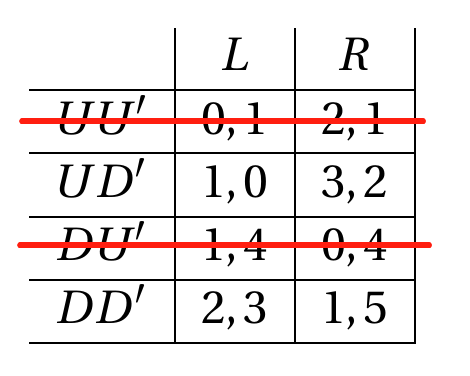
\includegraphics[width=0.4\textwidth]{9.q1}
\vspace{2mm}
\end{center}

\medskip

$(UD',R)$ is the unique NE.

\begin{mdframed}[backgroundcolor=blue!20,linecolor=white]
$UD'$ dominates $UU'$; $DD'$ dominates $DU'$ $\Rightarrow \ R$ dominates $L \ \Rightarrow \ UD'$ dominates $DD'$. 

\medskip

Dominated strategies can't be BR and should be assigned with probability 0 (no mixed-strategy NE).
\end{mdframed}

%%%%%%%%%%%%%%%%%%%%%%%%%%%%%%%%%%%%%%%%%%%%%%%%%%%%%%%%%%%%%%%%%%%%%%%%%%%%%%%%%%%%%%%%%%%%%%
\section{Problem 2 - Bayesian normal form}

Consider the following two variants of a battle-of-the-sexes game. The game at the top --
variant (i) -- is of the usual kind where both players wish to meet each other, while the one
at the bottom -- variant (ii) -- has the unusual feature that $1$ wishes to avoid 2.\vspace{-6pt}

% \begin{center}
% Variant (i) \vspace{6pt}

% $
% \begin{array}{c|c|c|}
%  & O & M \\
% \hline
% O & 3,1 & 0,0 \\
% \hline
% M & 0,0 & 1,3 \\
% \hline
% \end{array}
% $
% \end{center}

% \begin{center}
% Variant (ii) \vspace{6pt}

% $
% \begin{array}{c|c|c|}
%  & O & M \\
% \hline
% O' & 0,1 & 3,0 \\
% \hline
% M' & 1,0 & 0,3 \\
% \hline
% \end{array}
% $
% \end{center}
\begin{center}
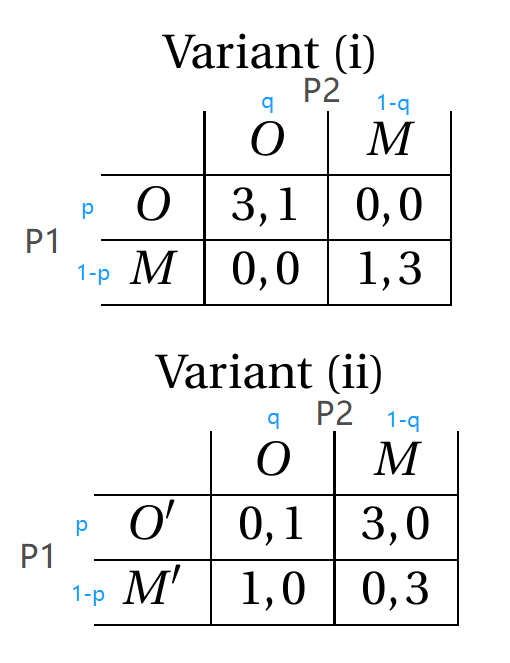
\includegraphics[width=0.4\textwidth]{9.q2}
\vspace{2mm}
\end{center}

%
\subsection*{(a) NE - static \& complete information}
For each of these games, determine the set of (pure) rationalizable strategies for each
player, and the set of pure-strategy and/or mixed-strategy NE.

\bigskip 

All strategies are rationalizable. 

\begin{mdframed}[backgroundcolor=blue!20,linecolor=white]
Recall: Rationalizable strategies(Watson pp.70): The set of strategies that
survive iterated dominance is therefore called the rationalizable strategies.

Here all strategies can be BR (= UD for 2-player games).
\end{mdframed}


\textbf{Variant (i)} has 2 pure NE $(O,O)$, $(M,M)$,  and a mixed NE $\left( \left( \tfrac34, \tfrac14 \right), \left( \tfrac14, \tfrac34 \right) \right)$ .

\medskip

To derive the mixed-strategy NE, let $p$ be the probability of $P_1$ choosing $O$ and $q$ be the probability of $P_2$ choosing $O$. 

$$U^1_O=3q$$ 
$$U^1_M=1-q$$

$$U^1_O = U^1_M \Rightarrow 3q = 1-q \Rightarrow q = \tfrac14$$

$$U^2_O=p$$ 
$$U^2_M=3(1-q)$$

$$U^2_O = U^2_M \Rightarrow p = 3(1-p) \Rightarrow p = \tfrac34)$$

\bigskip

\textbf{Variant (ii)}  has no pure NE but a mixed NE $\left( \left( \tfrac34, \tfrac14 \right), \left( \tfrac34, \tfrac14 \right) \right)$.

\medskip

To derive the mixed-strategy NE in variant (ii), let $p$ the probability of $1$ choosing $O'$ and $q$ being the probability of $2$ choosing $O$. 
$$U^1_O=3(1-q)$$ 
$$U^1_M=q$$
$$U^1_O = U^1_M \Rightarrow 3(1-q) = q \Rightarrow q = \tfrac34$$
$$U^2_O=p$$ 
$$U^2_M=3(1-p)$$
$$U^2_O = U^2_M \Rightarrow p = 3(1-p) \Rightarrow p = \tfrac34$$
\begin{mdframed}[backgroundcolor=blue!20,linecolor=white]
Recall: why players are indifferent between O and M in a Mixed strategy?
\end{mdframed}


%***************************************************

\subsection*{(b) Bayesian normal form}

Assume next that only player $1$ knows which game is being played, while player $2$ thinks that
the two games are equally likely. Model this situation in an \textit{ex ante} perspective by specifying
the Bayesian normal form.

\smallskip

\begin{mdframed}[backgroundcolor=blue!20,linecolor=white]
Think: Who has private information and therefore contingent strategies?

\medskip

Payoff is calculated similarly to Question 1. For example, for $(OO',O)$ is $(\tfrac32,1)$:

$$U^1 = 0.5 \times 3 + 0.5 \times 0 = \tfrac32$$
$$U^2 = 0.5 \times 1 + 0.5 \times 1 = 1$$
\end{mdframed}


\begin{center}
$
\begin{array}{c|c|c|}
 & O & M \\
\hline
OO' & \tfrac32,1 & \tfrac32,0 \\
\hline
OM' & 2,\tfrac12 & 0,\tfrac32 \\
\hline
MO' & 0,\tfrac12 & 2,\tfrac32 \\
\hline
MM' & \tfrac12,0 & \tfrac12,3 \\
\hline
\end{array}
$
\end{center}
%

%***************************************************

\subsection*{(c) Rationalizable strategies and NE}

For the Bayesian normal form found in part (b), determine the set of
(pure) rationalizable strategies for each player, and the set of pure-strategy and/or
mixed-strategy NE.

\bigskip

$MM'$ is dominated by $OO'$.
All the other strategies are rationalizable.

\medskip

\textbf{NE}: $(MO', M)$, $\left( \left( \tfrac12, \tfrac12, 0, 0 \right), \left( \tfrac34, \tfrac14 \right) \right)$, and $\left( \left( \tfrac12, 0, \tfrac12, 0 \right), \left( \tfrac14, \tfrac34 \right) \right)$. 

\medskip

For mixed stategy, $P_1$ chooses strategies among (note MM' is dominated and can't be chosen):

\begin{equation}
    \begin{cases}
OO' \\ OM' \\ MO'
    \end{cases}
\nonumber
\end{equation}

There are 4 possible combinations:

\begin{equation}
(1)
    \begin{cases}
OO' \\ OM'
    \end{cases}
\quad (2)
    \begin{cases}
 OM' \\ MO'
    \end{cases}
 \quad (3) 
    \begin{cases}
OO'  \\ MO'
    \end{cases}
 \quad (4) 
    \begin{cases}
OO' \\ OM' \\ MO'
    \end{cases}
\nonumber
\end{equation}

Let $q$ being the probability of $P_2$ choosing $O$.
\begin{align*}
U^1_{OO'} &= \tfrac32 q + \tfrac32 (1-q) = \tfrac32 \\
U^1_{OM'} &= 2 q + 0 \times (1-q) = 2q \\
U^1_{MO'} &= 0 \times q +  2 (1-q) = 2 (1-q) \\
\end{align*}


\medskip

\textbf{(1)} If $P_1$ mixes $OO'$ and $OM'$ with probability $(p,1-p)$, i.e. player 2 has belief $(p,1-p,0,0)$.
\medskip

For $P_1$:

$$U^1_{OO'} = U^1_{OM'} \Rightarrow \tfrac32 = 2q  \Rightarrow  q =\tfrac34$$

For $P_2$:

\begin{align*}
U^2_{O} &= p + \tfrac12 (1-p) \\
U^2_{M} &= 0 \times p + \tfrac32 (1-p) = \tfrac32 (1-p) \\
U^2_{O} &= U^2_{M} \Rightarrow p + \tfrac12 (1-p) =  \tfrac32 (1-p) \Rightarrow p=\tfrac12
\end{align*}


The NE is :$[\left( \tfrac12, \tfrac12, 0, 0 \right), \left( \tfrac34, \tfrac14 \right)]$


\begin{mdframed}[backgroundcolor=blue!20,linecolor=white]
Note how we assign 0 probability to the strategies $P_1$ doesn't choose.
\end{mdframed}

\textbf{(2)} If $P_1$ mixes $OM'$ and $MO'$ with probability $(p,1-p)$, i.e. player 2 has belief $(0,p,1-p,0)$.

\medskip

For $P_2$, facing with $P_1$'s mixed strategy, $M$ dominates $O$ (therefore $q=1$).
The mixed strategy brokes down (player 2's belief $(0,p,1-p,0)$ is not reasonable).

\medskip

\textbf{(3)} If $P_1$ mixes $OO'$ and $MO'$ with probability $(p,1-p)$, i.e. player 2 has belief $(p,0,1-p,0)$.
\medskip

For $P_1$:

$$U^1_{OO'} = U^1_{MO'} \Rightarrow \tfrac32 =  2 (1-q)  \Rightarrow  q =\tfrac14$$

For $P_2$:
\begin{align*}
U^2_{O} &= p + \tfrac12 (1-p) \\
U^2_{M} &= 0 \times p + \tfrac32 (1-p) = \tfrac32 (1-p) \\
U^2_{O} &= U^2_{M} \Rightarrow p + \tfrac12 (1-p) = \tfrac32 (1-p) \Rightarrow p=\tfrac12 \\
\end{align*}


The NE is :$[\left( \tfrac12, 0, \tfrac12, 0 \right), \left( \tfrac14, \tfrac34 \right)]$

\medskip

\textbf{(4)} If $P_1$ mixes $OO'$, $OM'$ and $MO'$ with probability $(m,n,1-m-n)$, i.e. player 2 has belief $(m,n,1-m-n,0)$.
\medskip

There must be $U^1_{OO'} = U^1_{OM'} = U^1_{MO'}$.

From (1) and (3) we already know 
$P_2$'s belief supporting $U^1_{OO'} = U^1_{OM'}$ is different from his/her belief supporting
$U^1_{OO'} = U^1_{MO'}$. Therefore there is no such a brief that supports
$U^1_{OO'} = U^1_{OM'} = U^1_{MO'}$ simultaneously.


\newpage

%%%%%%%%%%%%%%%%%%%%%%%%%%%%%%%%%%%%%%%%%%%%%%%%%%%%%%%%%%%%%%%%%%%%%%%%%%%%%%%%%%%%%%%%%%%%%%
\section{Problem 3 - Rationalizability in incomplete information games}

(Watson Exercise 26.3, solution is on pp.~469-470)

Suppose that nature selects A with probability $1/2$ and B with probability
$1/2$. If nature selects A, then players $1$ and $2$ interact according to matrix
``A.'' If nature selects B, then the players interact according to matrix ``B.''
These matrices are pictured here. Suppose that, before the players select
their actions, player $1$ observes nature's choice. That is, \textbf{player $1$ knows
from which matrix the payoffs are drawn}, and player $1$ can condition his
or her decision on this knowledge. Player $2$ does not know which matrix is
being played when he or she selects between L and R.

\begin{center}
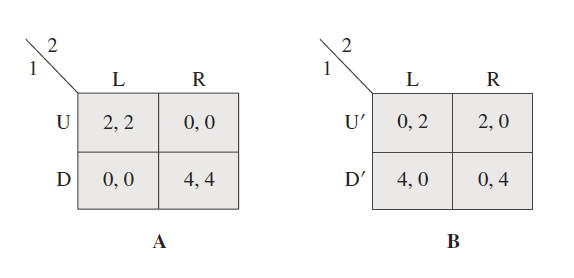
\includegraphics[width=0.7\textwidth]{9.q26_3}
\end{center}
\vspace{2mm}



\subsection*{(a) Representation, rationalizability and NE} 

\textbf{(1) Draw the extensive-form and Bayesian normal form. }

\begin{center}
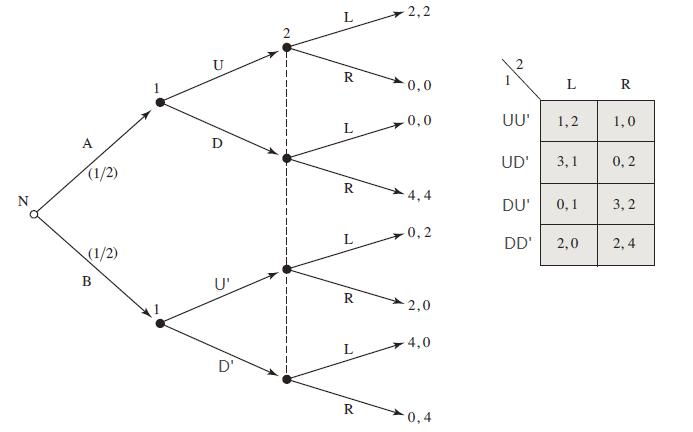
\includegraphics[width=0.9\textwidth]{9.q26_3_a}
\end{center}
\vspace{2mm}


\begin{mdframed}[backgroundcolor=blue!20,linecolor=white]
Note, the dashed line passes through all the four nodes, meaning player 2 doesn't know either which game is played (incomplete) or how player 1 moves (static), thus can only choose $L$ or $R$.
\end{mdframed}


\textbf{(2) Compute the set of rationalizable strategies and NE}
\vspace{2mm}

$UU'$ is dominated by $DD'$, then $L$ is dominated by $R$. In the end, only $(DU',R)$ survives iterated dominance method. 
\vspace{2mm}

Therefore the set of rationalizable strategies is $\{(DU',R)\}$. The only NE is $(DU',R)$

\subsection*{(b) A three-player interpretation } 

Consider a three-player interpretation of this strategic setting in which each of player 1's types is modeled as a separate player. That is, the
game is played by players 1A, 1B, and 2. Assume that player 1A's
payoff is zero whenever nature chooses B; likewise, player 1B's payoff
is zero whenever nature selects A. Depict this version of the game in the
\textbf{extensive form} (remember that payoff vectors consist of three numbers)
and in the \textbf{normal form}. Compute the set of \textbf{rationalizable strategies and
find the NE}.

\vspace{4mm}

Extensive form:

\begin{center}
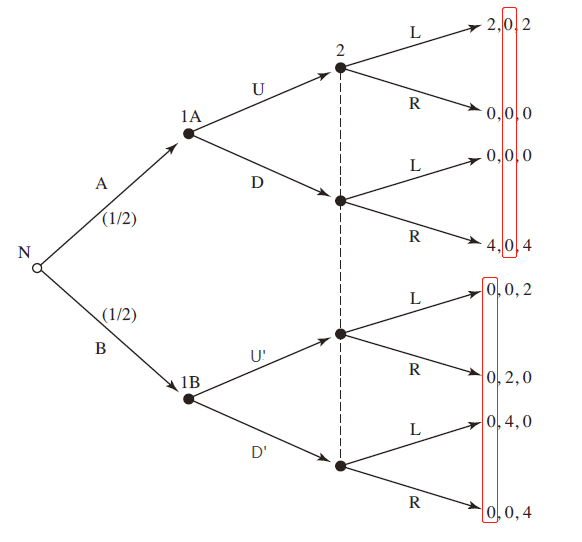
\includegraphics[width=0.7\textwidth]{9.q26_3_b1}
\end{center}
\vspace{2mm}

\begin{mdframed}[backgroundcolor=blue!20,linecolor=white]
Player 2 doesn't who he/she is playing with.
\vspace{2mm}

Note also when Player 1A (1B) is reached, the payoff for 1B (1A) is 0 (in red frame).
\end{mdframed}


\vspace{4mm}

Normal form:

\begin{center}
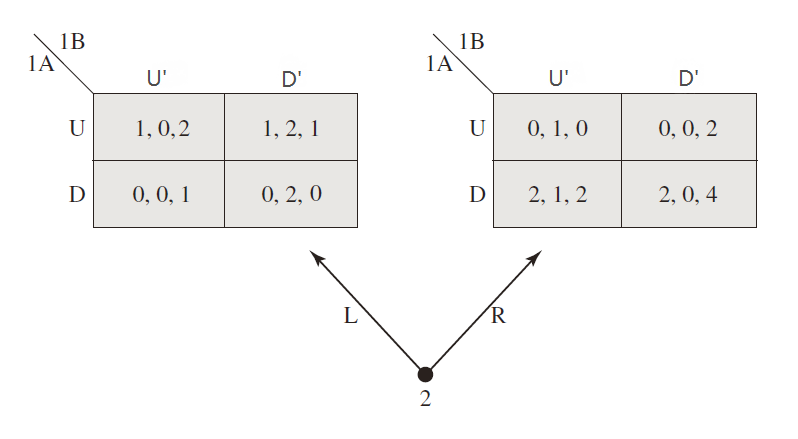
\includegraphics[width=0.7\textwidth]{9.q26_3_b2}
\end{center}
\vspace{2mm}

\begin{mdframed}[backgroundcolor=blue!20,linecolor=white]
Although there are 3 players, player 2 still doesn't know who he/she is playing with. As a result, the payoff is in player 2's imagination, and player $1A$,$1B$ know how player 2 thinks clearly (an \textit{ex ante} perspective).

\medskip

You can also draw the normal form the way on Geir's slides (lecture part 5, pp.5), i.e. draw
the matrix for player $1B$ and player $2$, and player $1A$ joins as another player. 

\begin{itemize}
\item We use the textbook's way because it makes the next question more clearly,
\item Note also the difference between the textbook and Geir's slides:
\begin{itemize}

\item The textbook calculates expected payoff for all the 3 players,  It's more intuitive and can get the correct Bayesian NE.

\item The slides pp.5 is an \textit{ex post} perspective, and the payoff for player $1A$ and $1B$ is not expected payoff but what they can really get. The result should be the same.

\item More about \textit{ex post} and \textit{ex ante} perspective can be found \href{https://www.cs.toronto.edu/~cebly/2534/Notes/CSC2534_Lecture9.pdf}{here}.
\end{itemize}

\end{itemize}

\end{mdframed}

\subsubsection*{Rationalizable strategies}
\vspace{2mm}

\textbf{For player $1A$ and $1B$:}

When player $2$ choose $L$,  $D'$ dominates $U'$, and $U$ dominates $D$. (($U$,$D'$) survives iterated dominance)

When player $2$ choose $R$, $D$ dominates $U$, and  $U'$ dominates $D'$. (($D$,$U'$) survives iterated dominance)

As a result, all the strategies for $1A$ and $1B$ can be BR.

\medskip

\textbf{For Player $2$:} 

Neither $L$ nor $R$ is dominated by the other action. Therefore both of the two 
actions are rationalizable.

\medskip

\textbf{In conclusion}: the rationalizable strategy set is: $\{(U,D),(U',D'),(L,R)\}$.

\subsubsection*{Find the NE}
By backward induction, if player $2$ chooses $L$, the payoff is $1$ (by $(U,D',L)$); if player $2$ chooses $R$, the payoff is $2$ (by $(D,U',R)$). Thus player $2$ will choose $R$ and the NE is $(D,U',R)$.

\begin{mdframed}[backgroundcolor=blue!20,linecolor=white]
Note although player $2$ will only choose $R$ by backward induction, $R$ doesn't dominate $L$. Dominance means "always better no matter how the opponents act". Obviously, under some conditions $L$ yields more payoff than $R$.
\end{mdframed}



\subsection*{(c) 2-player view \& 3-player view}
Explain why the predictions of parts (a) and (b) are the same in regard
to equilibrium but different in regard to rationalizability. (Hint: The
answer has to do with the scope of the players' beliefs.)


\begin{mdframed}[backgroundcolor=blue!20,linecolor=white]
In the Bayesian normal form (in part(a)), $DD'$ strictly dominates $UU'$. That means that $DD'$ is better than $UU'$ independently of what beliefs player $1$ has about the choice of player 2. 

This is true because player $1$ is one person and has a coherently belief. 

\medskip

If we use the view of 3 players, then palyer $1$ are 2 different people, then $(DD',L)$ means both player $1A$ and player $1B$ think player $2$ will choose $L$, and $(DD',R)$ means both player $1A$ and $1B$ think player 2 will choose $R$.

\medskip

What if player $1A$ and player $1B$ have different belief? For example, player $1A$ believes player $2$ chooses $L$, then $U$ is prefered; and at the same time, player $1B$ believes player $2$ chooses $R$, then $U'$ is prefered.
\medskip

In this case, (U,U') is chosen separetely, not dominated!

\medskip

This belief separation  doesn't affect NE because both player $1A$ and player $1B$ must agree that by backward induction, player $2$ will choose $R$. 
\end{mdframed}

In part (b), the beliefs of players $1A$ and $1B$ do not have to
coincide, so they may end up making $U$ and $U'$ as rational choices based on their separated beliefs. While in NE, the beliefs of player $1A$ and $1B$ are the same (by backward induction).


\newpage
%%%%%%%%%%%%%%%%%%%%%%%%%%%%%%%%%%%%%%%%%%%%%%%%%%%%%%%%%%%%%%%%%%%%%%%%%%%%%%%%%%%%%%%%%%%%%%
\section{Problem 4 - Differentiated duopoly}

(Watson Exercise 26.5,  solution is on pp.~470.)

Consider a differentiated duopoly market in which firms compete by selecting
prices and produce to fill orders. Let $p_1$ be the price chosen by firm
1 and let $p_2$ be the price of firm 2. Let $q_1$ and $q_2$ denote the quantities demanded
(and produced) by the two firms. Suppose that the demand for firm
1 is given by $q_1 = 22 - 2p_1 + p_2$ , and the demand for firm $2$ is given by
$q_2 = 22 - 2p_2 + p_1$ . Firm $1$ produces at a constant marginal cost of 10 and
no fixed cost. Firm $2$ produces at a constant marginal cost of c and no fixed
cost. The payoffs are the firms' individual profits.

\subsection*{(a) Payoff functions} The firms' strategies are their prices. Represent the normal form by writing the firms' payoff functions.

\begin{align*}
U^1 &= p_1 q_1 - 10 q_1 \\
&= p_1(22 - 2p_1 + p_2) -10(22 - 2p_1 + p_2) \\
&= 22P_1 -2p_1^2 + p_1p_2 - 220 + 20p_1 -10p_2 \\
&= -2p_1^2 +p_1p_2 + 42p_1 - 10p_2 -220\\
\\
U^2 &= p_2 q_2 - c q_2 \\
&= p_1(22 - 2p_2 + p_1) -c(22 - 2p_2 + p_1) \\
&= 22P_2 -2p_2^2 + p_1p_2 - 22c + 2cp_2 -cp_1 \\
&= -2p_2^2 +p_1p_2 -cp_1 + (22+2c)p_2 -22c
\end{align*}

\subsection*{(b) Calculate the firms' best-response functions.} 

FOC:

$$\frac{\partial U^1}{\partial p_1} = 0 \Rightarrow -4p^*_1+42+p_2 = 0 \Rightarrow p^*_1 = \frac{42+p_2}{4}$$

SOC:

$$\frac{\partial^2 U^1}{\partial p^2_1} = -4 <0$$

FOC:

$$\frac{\partial U^2}{\partial p_2} = 0 \Rightarrow -4p^*_2+22+2c+p_1 = 0 \Rightarrow p^*_2 = \frac{22+2c+p_1}{4}$$

SOC:

$$\frac{\partial^2 U^2}{\partial p^2_2} = -4 <0$$

\begin{mdframed}[backgroundcolor=blue!20,linecolor=white]
For payoff functions, we use FOC \& SOC to find the BR functions. Be clear about what is variable an what is parameter. See also seminar 7 problem 3.
\end{mdframed}

\subsection*{(c) Complete information} Suppose that $c = 10$ so the firms are identical (the game is symmetric). Calculate the NE prices.

\medskip

When $c = 10$, we have:

\begin{align*}
p^*_1 = \frac{42+p_2}{4} \\
p^*_2 = \frac{42+p_1}{4}
\end{align*}

NE is a price s.t. both of the two firms are applying BR and there is no incentive to devicate.
That is, $p^*_1 = \frac{42+p^*_2}{4} =\frac{42+\frac{42+p_1}{4}}{4}$ (or $p^*_2 = \frac{42+p^*_1}{4}$).

Therefore $p^*_1 = p^*_2 =14$.

\subsection*{(d) Incomplete information} Now suppose that firm $1$ does not know firm 2's marginal cost c. With
probability $1/2$ nature picks $c = 14$, and with probability 1/2 nature
picks $c = 6$. \textbf{Firm $2$ knows} its own cost (that is, it observes nature's
move), but firm $1$ only knows that firm 2's marginal cost is either $6$ or
$14$ (with equal probabilities). Calculate the best-response functions of
player $1$ and the two types ($c = 6$ and $c = 14$) of player $2$ and calculate
the Bayesian NE quantities.

\bigskip

\begin{mdframed}[backgroundcolor=blue!20,linecolor=white]
With different MC, firm 2 can set different (contingent) price, while firm 1 can only set one price according to its expected payoff function.
\medskip

(Compare this with the extensive from games in this seminar. Always be clear about who has contingent strategies!)

\end{mdframed}

\textbf{For firm 2:}

\medskip

\textbf{$\quad $ (1) When $c=c^H=14$}

\smallskip

$\quad $(I omitted the superscript $^H$ of $p_2$ and $c$ for simpliciy. )
\begin{align*}
U^{2H} &= -2p_2^2 +p_1p_2 -cp_1 + (22+2c)p_2 -22c \quad \quad \text{(the result from question a.)}  \\
&= -2p_2^2 +p_1p_2 -14p_1 + 50p_2 -22 \times 14
\end{align*}

$\quad $FOC:

$$\frac{\partial U^{2H}}{\partial p_2} = 0 \Rightarrow -4p^{H*}_2+ 50 + p_1 = 0 \Rightarrow p^{H*}_2 = \frac{50+p_1}{4}$$

$\quad $SOC:

$$\frac{\partial^2 U^{2H}}{\partial p^2_2} = -4 <0$$



\textbf{$\quad $(2)When $c=c^L=6$}

\smallskip

$\quad $ (I omitted the superscript $^L$ of $p_2$ and $c$ for simpliciy.)

\begin{align*}
U^{2L} &= -2p_2^2 +p_1p_2 -cp_1 + (22+2c)p_2 -22c \quad \quad \text{(the result from question a.)}  \\
&= -2p_2^2 +p_1p_2 -6p_1 + 34p_2 -22 \times 6
\end{align*}


$\quad $FOC:

$$\frac{\partial U^{2L}}{\partial p_2} = 0 \Rightarrow -4p^{L*}_2+ 34 + p_1 = 0 \Rightarrow p^{L*}_2 = \frac{34+p_1}{4}$$

$\quad $SOC:

$$\frac{\partial^2 U^{2L}}{\partial p^2_2} = -4 <0$$



\textbf{For firm 1:}

\begin{align*}
E(U^1)&= 0.5 U^1(p_1,p_2^H) + 0.5 U^1(p_1,p_2^L) \\
&= 0.5(-2p_1^2 +p_1p^H_2 + 42p_1 - 10p^H_2 -220) + 0.5(-2p_1^2 +p_1p^L_2 + 42p_1 - 10p^L_2 -220)\\
&=-2p_1^2 + 42p_1 +(p_1 -10)(0.5p^H_2 + 0.5p^L_2) -220
\end{align*}

\begin{mdframed}[backgroundcolor=blue!20,linecolor=white]
Can we substitute firm 2's BR ($p^{H*}_2, p^{L*}_2$) into firm 1's expected utility function now? No! We want to get firm 1's BR to any ($p^H_2, p^L_2$), not just to firm 2's BR ($p^{H*}_2, p^{L*}_2$)!
\end{mdframed}


$\quad $FOC:

$$\frac{\partial U^{1}}{\partial p_1} = 0 \Rightarrow -4p^{*}_1+ 42 +(0.5p^H_2 + 0.5p^L_2) = 0 \Rightarrow p^{*}_1 = \frac{42 + 0.5(p^H_2 + p^L_2)}{4}$$

$\quad $SOC:

$$\frac{\partial^2 U^{1}}{\partial p^2_1} = -4 <0$$


\textbf{NE}: Denote the NE as $(p^*_1,p^{*H}_2,p^{*L}_2)$, we have


$$p^{*}_1 = \frac{42 + 0.5(p^{*H}_2 + p^{*L}_2)}{4}= \frac{42 + 0.5(\frac{50+p_1}{4} + \frac{34+p_1}{4})}{4} $$

Therefore: 

\begin{equation}
    \begin{cases}
p^*_1 = 14 \\ p^{*H}_2 = 16 \\ p^{*L}_2 =12
    \end{cases}
\nonumber
\end{equation}







\end{document}
